\documentclass{article} \usepackage{amsmath} \usepackage{amssymb} \usepackage{amsthm} \usepackage[margin=0.2in]{geometry} \usepackage{hyperref} \usepackage{physics} \usepackage{tikz} \usepackage{mathtools} \mathtoolsset{showonlyrefs} \theoremstyle{definition} \newtheorem{theorem}{Theorem}[section] \newtheorem{corollary}{Corollary}[theorem] \newtheorem{lemma}[theorem]{Lemma} \newtheorem{definition}{Definition}[section] \author{Connor Duncan} \date{\today}
\title{Physics-105-Lecture-Notes-03-12-2019}
\begin{document}
\maketitle\tableofcontents
\noindent\abstract{A single PDF with all lectures in a single document can be downloaded at \url{https://www.dropbox.com/sh/8sqzvxghvbjifco/AAC9LoSRnsRQDp7pYedgWpQMa?dl=0}. The password is 'analytic.mech.dsp'.
 This file was automatically generated using a script, so there might be some errors. If there are, you can contact me at \url{mailto:ctdunc@berkeley.edu}.}
\subsection{Canonical Transformations (not in book)} There's some discussion of this in Hand + Finch. We have some $H(q,p,t)$, where $p$ is the canonical momentum. \begin{align} \dot p=-\pdv{H}{q}\\ \dot q=\pdv{H}{p} \end{align} If we have a cyclic coordinate, it simplifies the problem, i.e. if $\pdv{H}{q}=0$, then $\dot p=0\Rightarrow p$ is a constant. Good example of this principle is central force problems, since $\mathcal L=\frac{1}{2}m\dot r^2+r^2\dot\theta^2-V(r)$, potential exclusively depends on $r$, which means $\pdv{L}{\theta}=0\rightarrow l=mr^2\dot\theta\equiv$ constant. Canonical Transformations are ways of finding convenient coordinates to make the hamiltonian cyclic as well. Lets call the transform $Q=Q(p_i,q_i,t)$, and $P=P(q_i,p_i,t)$. If it makes some $\mathcal H$ cyclic in $Q$, then $\mathcal H=\mathcal H(P)$, which implies $\dot Q=\pdv{\mathcal H}{P}=\omega\equiv$ constant, $Q=\omega t+Q_0$, $\dot p=-\pdv{\mathcal H}{Q}=0$, $p\equiv$const. $(q,p)$ are called canonically conjugate, that if Hamiltons equations hold for $(q,p)\Leftrightarrow(Q,P)$ under canonical equations. Hamiltons Principle \begin{align} \delta\int L(q,\dot q,t)dt=0=\delta\int\mathcal L(Q,\dot Q,t)dt \end{align} this means that $\delta(L-\mathcal L)dt=0$. Because this is a time integral, the lagrangian and the transformed lagrangian can differ by a total differential and this would still be true. \begin{equation} \delta\int_{t_1}^{t_2}\dv{F}{t}dt=\delta\left(F(t_2)-F(t_1)\right)=0 \end{equation} which implies that \begin{equation} L-\mathcal L=\dv{F}{t} \end{equation} with $F$ called the \textbf{generating function}. It should have $2n+1$ independent variables. There are four types of generating functions \begin{align} F_1=F(q_i,Q_i,t)\\ F_2=F(q_i,P_i,t)\\ F_3=F(p_i,Q_i,t)\\ F_4=F(p_i,P_i,t) \end{align} going back to transformed lagrangian, we take $L=\mathcal K+\dv{F}{t}=\sum p\dot q-H$, we can write this as \begin{align} \sum p\dot q-H=\sum P\dot Q-\mathcal H+\dv{F}{t} \end{align} \subsubsection{Type 1 Generator} This gives that \begin{equation} \dv{F_1}{t}=\pdv{F_1}{q}\dot q+\pdv{F_1}{Q}\dot Q+\pdv{F_1}{t} \end{equation} This can be expressed as \begin{align} \sum p\dot q-\sum P\dot Q-H+\mathcal H=\sum\pdv{F_1}{q}\dot q+\sum\pdv{F_1}{Q}\dot Q+\pdv{F_1}{t} \end{align} which gives that \begin{align} p_i=\pdv{F_1}{q_i}(q_i,Q,t)\\ P_i=-\pdv{F_1}{Q}(q,Q,t)\\ \mathcal H=H+\pdv{F_1}{t}(q,Q,t) \end{align} \subsubsection{2 Examples} \paragraph{Coordinate Swap} take $F_1(q,Q)=qQ$. Then \begin{align} p_i=\pdv{F}{q}=Q\\ P_i=-\pdv{F}{Q}=-q \end{align} \paragraph{Simple Harmonic Oscillator} Recall $L=\frac{1}{2}m\dot q^2+\frac{1}{2}kq^2$, which gives \begin{align} p=\pdv{L}{\dot q}=m\dot q\rightarrow q=\frac{p}{m}\\ H=\frac{1}{2m}(p^2+m^2\omega^2q^2)\\ \omega^2=\frac{k}{m} \end{align} Let's try this: \begin{align} p=f(P)\cos(Q)\\ q=\frac{f(P)}{m\omega}\sin(Q) \end{align} if we put these into the old hamiltonian, we get \begin{equation} p^2+m^2\omega^2q^2=f(P)^2\cos^2(Q)+f(P)^2\sin^2(Q)=f(P)^2 \end{equation} which gives our new hamiltonian as \begin{equation} \mathcal H=\frac{f(P)^2}{2m} \end{equation} Let's get a new type one generator as defined above, so that \begin{align} p=\pdv{F}{q}\\ P=-\pdv{F}{Q} \end{align} Carrying on with the hamiltonian that we already have, we get \begin{align} p=m\omega q\cot Q=\pdv{F}{q} \end{align} which gives that \begin{equation} F=\int pdq=\frac{1}{2}m\omega q^2\cot Q \end{equation} it is also easy to see that $p=-\pdv{F}{Q}=\frac{1}{2}m\omega^2q^2\frac{1}{\sin^2(Q)}$, \begin{align} q=\sqrt{\frac{2P}{m\omega}}\sin(Q)\\ p=m\omega\sqrt{\frac{2P}{m\omega}}\cos(Q) \end{align} putting this all into the hamiltonian, we have \begin{align} H=\frac{1}{2m}\left[2Pm\omega\cos^2Q+m\omega2P\sin^2Q\right] \end{align} which gives, cancelling out, that \begin{equation} \mathcal H=\omega P \end{equation} since we knnow it doesn't depend on time, we can write that \begin{equation} E\equiv\mathcal H=\omega P \end{equation} so $P=\frac{E}{\omega}$, or energy per unit angular momentum, so we have that $\dot Q=\omega$, which gives \begin{equation} Q=\omega t+Q_0 \end{equation} Putting these back into the original solution, we find that \begin{align} p=\sqrt{2mE}\cos(\omega t+Q_0)\\ q=\sqrt{\frac{2E}{m\omega^2}}\sin(\omega t+Q_0) \end{align} Let's look at phase space! \begin{center} 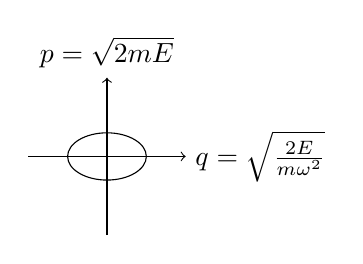
\begin{tikzpicture} \draw[->] (0,-1)--(0,1) node[anchor=south]{$p=\sqrt{2mE}$}; \draw[->] (-1,0)--(1,0) node[anchor=west]{$q=\sqrt{\frac{2E}{m\omega^2}}$}; \draw (0,0) ellipse (0.5 and 0.3); \end{tikzpicture} $\Leftrightarrow$ \begin{tikzpicture} \draw[->] (0,-1)--(0,1) node[anchor=south]{$P$}; \draw[->] (-1,0)--(1,0) node[anchor=west]{$Q$}; \draw (0,0) rectangle (0.7,0.7)--(1,0.7) node[anchor=west]{$E/\omega$}; \end{tikzpicture} \end{center} \section{Rigid Body Motion} \definition A rigid body is a body in which the mass elements are fixed with respect to one another. \begin{center} \begin{tikzpicture} \draw[->] (-2,0)--(2,0)node[anchor=west]{$\omega$}; \draw plot [smooth] coordinates {(-1,0)(-0.5,-0.6)(0,-1)(0.5,-0.43)(1,0)(0.5,0.8)(0,1)(-0.5,0.4)(-1,0)}; \draw[fill] (0,0) ellipse (0.02) node[anchor=south]{$p$}; \end{tikzpicture} \end{center} We have $\vec{L}=\vec{r}\times\vec{p}$, and $p=m\omega$, with point $p$ rotating at an angle $\theta$ away from $\omega$, and momentum $p$ at $r'=r\sin\theta$ along that vector Some mass element $\delta m$, we get $\delta\vec{L}=\vec{r}\times\delta\vec{p}=\vec{r}\times\vec{v}\delta m$, which gives \begin{equation} \vec{L}=\int\delta m(\vec{r}\times(\vec{\omega}\times\vec{r}) \end{equation} or for discrete mass elements, we have \begin{equation} \vec{L}=\sum_im_i\vec{r}_i\times(\omega\times\vec{r}_i) \end{equation} Then, we actually do the cross product out, we get \begin{align} \vec{\omega}\times\vec{r}=(\omega_2z-\omega_3y)\hat x+(\omega_3x-\omega_1z)\hat y+(\omega_1y-\omega_2x)\hat z \end{align} , so the whole thing comes out to be, after crossing with $r$ again, \begin{equation} \begin{bmatrix}L_1\\L_2\\L_3\end{bmatrix} = \begin{bmatrix} \int(y^2+z^2)dm&-\int xydm&-\int zxdm\\ -\int xydm&\int(z^2+x^2)dm&-\int yzdm\\ -\int zxdm&-\int yzdm&\int(x^2+y^2)dm \end{bmatrix} \begin{bmatrix}\omega_1\\\omega_2\\\omega_4\end{bmatrix} \end{equation} with that big ol matrix defined as the \emph{Inertia Tensor}, $\vec{I}$. Inertia Tensor has a couple of properties \begin{itemize} \item Symmetric and Positive Definite. \item Depends only on the \emph{shape} of the system, not $\omega$. \item Can only be calculated after choosing an origin and coordinate system. \item Is diagnoalizable. \end{itemize} We could also write it in the following way, \begin{equation} I_{ij}=\int_{\text{all } V}\rho(\vec{r})\left(\delta_{ij}\sum_k(x_k)^2-x_ix_j\right)dV \end{equation} \subsection{ex: Point mass in a plane} Some mass orbiting $\hat z$ in the $x-y$ plane, $m$, wiht $\omega=(0,0,\omega_3)$ and $x^2+y^2=r^2$, we have \begin{align} \vec{L}=\begin{bmatrix} \int y^2 & -\int xy & 0\\ -\int xy & \int x^2 & 0\\ 0 & 0 & \int(x^2+y^2)dm \end{bmatrix} \begin{bmatrix}0\\0\\\omega_3\end{bmatrix} \\ = \begin{bmatrix}0\\0\\ \omega_3\int(x^2+y^2)dm \end{bmatrix} \end{align} which just reduces to $\vec{L}=mr^2\omega_3\hat z=mvr\hat z$, which is what we expected anyways. There's also the parallel axis theorem, which we will discuss later. \subsection{Kinetic Energy} We can also examine the kinetic energy, which is given by \begin{align} dT=m\frac{v^2}{2}=\frac{dm|\vec{\omega}\times{r}|^2}{2}\\ T=\frac{1}{2}\int\left((\omega_2z-\omega_3y)^2+(\omega_3x-\omega_1z)^2+(\omega_1y+\omega_3x)^2\right)dm\\ =\frac{1}{2}\vec{\omega}\cdot(\vec{I}\cdot\vec{\omega})=\frac{1}{2}\vec{\omega}\cdot\vec{L} \end{align} \subsection{Center of Mass Coordinates} Say $r=\vec{R}+\vec{r}'$, where $\vec{R}$ goes from origin to center of mass. we have \begin{align} \vec{L}=\int dm(\vec{r}\times\vec{v})=\int\left((\vec{R}+\vec{r}')\times(\vec{r}'+(\vec{\omega}\times\vec{r}'))\right)\\ (\vec{R}+\vec{r}')\times(\vec{V}+(\vec{\omega}\times\vec{r}')=\vec{r'}\times\vec{v}'+\vec{r}'\times(\vec{\omega}\times\vec{r}') \end{align} which gives that \begin{equation} \vec{L}=m\vec{R}\times \vec{V}+\vec{L}_{cm} \end{equation} We can also do this for KE, which would give us that \begin{align} T=\frac{1}{2}\int dmV^2=\frac{1}{2}\int dm|\vec{V}+(\vec{\omega}'\times\vec{r}')|^2\\ =\frac{1}{2}MV^2+\frac{1}{2}\vec{\omega}'\cdot\vec{L}_{cm} \end{align} \subsection{Principal Axes} Goal is to diagonalize the inertial tensor. \begin{equation} \vec{I}=\begin{bmatrix}I_1&0&0\\0&I_2&0\\0&0&I_3\end{bmatrix} \end{equation} where $I_1,I_2,I_3$ are defined as the principal moments. This kind of thing should be somewhat familiar from freshman mechanics classes, since we have something like a plate in $\mathbb{R}^3$, ortthogonal to the $z$ axis, the cross terms like $xydm$ cancel in the inertia tensor, but you get and eigenvalue problem. We want $\vec{L}=\vec{I}\cdot\vec{\omega_1}=I_1\omega_1$, or $\omega_1$ lies along a principal axis. Want \begin{align} \det\left|\begin{bmatrix} I_{xx}-I & I_{xy} & I_{xz}\\ I_{xy} & I_{yy}-I& I_{yz}\\ I_{xz} & I_{yz} & I_{zz}-I \end{bmatrix} \right|=0 \end{align} \subsubsection{Todo next lecture} \begin{center} 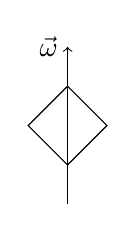
\begin{tikzpicture} \draw[->](0,-1)--(0,1) node[anchor=east]{$\vec{\omega}$}; \draw plot coordinates {(0,-0.5)(0.5,0)(0,0.5)(-0.5,0)(0,-0.5)}; \end{tikzpicture} \end{center}
\end{document}
